\section{Mallas dinámicas}
\label{walls_holes}
Uno de los principales requerimientos para un planificador es la visualización de paredes y configuración de estas para adaptarlas a las medidas de una estancia. Además, deben poderse ubicar ventanas y puertas en las paredes, lo cual afecta a la geometría de la pared dado que se debe poder ver a través de estos elementos. Para ello no es factible utilizar mallas pregeneradas, se necesita generar las paredes de forma dinámica.

En este apartado se describe el proceso de desarrollo de las paredes en 2 iteraciones, una primera en la que se crea una estructura básica para las paredes, y otra en la que se tienen en cuenta las ventanas y puertas.

%%%%%%%%%%%%%%%%%%%%%%%%%%%%%%%%%%%%%%%%%%%%%%%%%%%%%%%%%%%%%%%%%%%%%%%%%%%%%
%%%%%%%%%%%%%%%%%%%%%%%%%%%%%%%%%%%%%%%%%%%%%%%%%%%%%%%%%%%%%%%%%%%%%%%%%%%%%
%%%%%%%%%%%%%%%%%%%%%%%%%%%%%%%%%%%%%%%%%%%%%%%%%%%%%%%%%%%%%%%%%%%%%%%%%%%%%
\subsection{Generación de la estructura básica de la pared}
\label{subsec:gen1}
El primer paso ha sido crear una definición de los datos que se recibirán para describir cómo ha de ser la pared. Se trata de una lista de puntos en dos dimensiones y un valor booleano que indica si esta lista debe cerrarse conectando el último punto con el primero. Esto último es importante porque, como se puede ver en la figura \ref{fig:vertical_view_walls}, la geometría de una esquina ``suelta" es diferente a la de una esquina que conecta dos paredes entre sí.

\begin{figure}[h]
    \centering
    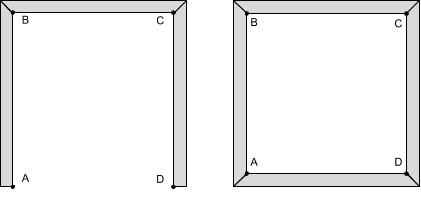
\includegraphics[width=0.65\linewidth]{Vista_Vertical_Paredes}
    \caption{Paredes en vista vertical.}
    \label{fig:vertical_view_walls}
\end{figure}

Estos datos nos permiten no sólo crear habitaciones sino también paredes únicas o incluso otros tipos de estructuras, normalmente interiores, similares a una pared. La intención es que en el futuro el programa pueda utilizarse en otras herramientas para hacer diseños más complicados como el plano de una planta completa de un edificio.

Teniendo en cuenta la estructura de una malla, explicada en el apartado \ref{mesh_light_cam}, en la figura \ref{fig:io_generatewalls} se puede ver la conversión de los datos que se espera conseguir.

\begin{figure}[H]
    \centering
    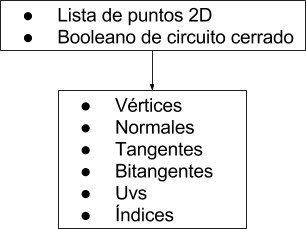
\includegraphics[width=0.5\linewidth]{IO_paredes}
    \caption{Input y output del generador de paredes.}
    \label{fig:io_generatewalls}
\end{figure}

El output está formado por listas de valores planos. Por ejemplo, la lista de vértices está formada por los valores de posición ``x,y,z" de cada uno sucesivamente.

Por cada pared hay tres primeros puntos 2D relevantes: las esquinas izquierda de las paredes anterior, actual, y siguiente. A partir de estos tres puntos puede deducirse la información de la figura \ref{fig:wall_vectors}, donde los vectores ``N1" y ``N2" son las normales de cada pared, siempre hacia el exterior de la estancia.

\begin{figure}[H]
    \centering
    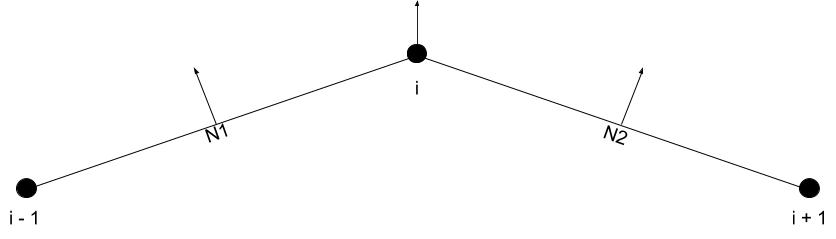
\includegraphics[width=\linewidth]{data_from_3_points}
    \caption{Vectores extraídos a partir de 3 puntos consecutivos.}
    \label{fig:wall_vectors}
\end{figure}

``N1" y ``N2" pueden obtenerse normalizando los vectores de un punto a otro, y girándolos. La dirección del vector central es la suma normalizada de estos dos o, en el caso de las paredes en los extremos cuando el circuito no está cerrado, la normal de la propia pared:

\begin{lstlisting}
VARIABLES EXTERNAS:
    puntos: lista de puntos 2D
    i: punto desde el que queremos obtener las normales de pared
    cerrado: booleano que indica si se quiere cerrar el conjunto de paredes

VARIABLE direccion TIPO VECTOR
VARIABLES v_pc, v_cn, normal_actual, normal_anterior TIPO VECTOR
VARIABLES actual, anterior, siguiente TIPO NUMERO

actual = i
anterior = i - 1

SI i EQUIVALE A tamaño(puntos) ENTONCES:
    siguiente = 0
SINO
    siguiente = i + 1
FINSI

v_pc = puntos[actual] - puntos[anterior];
v_cn = puntos[siguiente] - puntos[actual];

SI cerrado Y (actual EQUIVALE A tamaño(puntos) - 1 O actual EQUIVALE A 0) ENTONCES:
    normal_actual = GIRAR 90 GRADOS ANTI-HORARIO v_cn Y NORMALIZAR
    direccion = puntos[actual] + normal_actual
SINO
    normal_actual = GIRAR 90 GRADOS ANTI-HORARIO v_cn
    normal_anterior = GIRAR 90 GRADOS ANTI-HORARIO v_pc
    direccion = normal_actual + normal_anterior
    NORMALIZAR direccion
FINSI
\end{lstlisting}

Por último se debe tener en cuenta el grosor que se espera que tenga la pared, dado que si se avanza siempre la misma distancia en el vector director el grosor de estas dependería del ángulo que formen con sus paredes adyacentes. Esto se resuelve con trigonometría:

\begin{lstlisting}
SI cerrado ENTONCES:
    direccion = profundidad_pared / absoluto(producto_punto(normal_actual, direccion));
SINO
    direccion = profundidad_pared * normal_actual
FINSI

punto_esquina = puntos[actual] + direccion
\end{lstlisting}

El producto punto de dos vectores normales es el coseno del ángulo que forman entre sí. En este momento ``direccion" incluye la dirección y distancia entre el punto actual y el punto de la esquina exterior, permitiendo generar dicho punto a partir del actual. En el caso de que la pared que estamos generando no haga esquina con otra, simplemente se utiliza la normal de la pared actual.

Una limitación de este sistema es que los puntos deben introducirse en sentido anti-horario respecto al interior de la habitación. De lo contrario la normal de cada pared queda invertida y estas se extienden hacia el lado opuesto al que deberían, provocando algunos artefactos no deseados.

%%%%%%%%%%%%%%%%%%%%%%%%%%%%%%%%%%%%%%%%%%%%%%%%%%%%%%%%%%%%%%%%%%%%%%%%%%%%%
%%%%%%%%%%%%%%%%%%%%%%%%%%%%%%%%%%%%%%%%%%%%%%%%%%%%%%%%%%%%%%%%%%%%%%%%%%%%%
%%%%%%%%%%%%%%%%%%%%%%%%%%%%%%%%%%%%%%%%%%%%%%%%%%%%%%%%%%%%%%%%%%%%%%%%%%%%%
\subsection{Índices para la estructura básica}
Para referir a cada uno de los vértices se ha definido la nomenclatura ``A, B, A2, B2" como puede verse en la figura \ref{fig:nomenclatura_vertices}, además de los correspondientes ``AH, BH, A2H, B2H" en la parte alta de la pared. Posteriormente, los índices de la pared se extraen de los que habría normalmente en un cubo, aprovechando que sus vértices se conectan del mismo modo.

\begin{figure}[H]
    \centering
    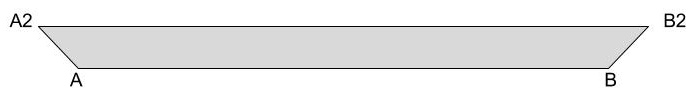
\includegraphics[width=0.75\linewidth]{Nomenclaturas_vertices}
    \caption{Nomenclatura básica de los vértices.}
    \label{fig:nomenclatura_vertices}
\end{figure}

La pared tiene 23 vértices y no 8 como cabría esperar. Esto se debe a que al renderizar, los shaders interpolan la normal de cada vértice con la de sus vecinos; si el mismo vértice se encuentra en dos caras distintas, la normal del vértice no coincide con la de la superficie en la cara que se está pintando. El resultado de esto sería que el color varía en los bordes de cada cara. Esta propiedad es muy útil para objetos que no tienen ángulos tan marcados, pero en este caso se busca que las caras sean muy marcadas y totalmente planas.

Para solucionarlo se repite cada vértice tantas veces como el número de caras en el que se encuentre, de modo que aunque todos se encuentren en la misma posición, cada cara está utilizando un vértice distinto.

\begin{figure}[H]
    \centering
    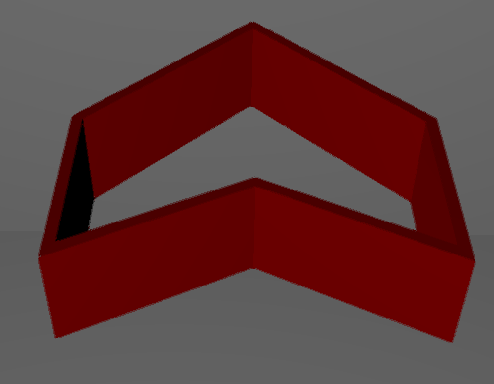
\includegraphics[width=0.75\linewidth]{paredes_first}
    \caption{Ejemplo de generación de paredes.}
    \label{fig:paredes_first}
\end{figure}

%%%%%%%%%%%%%%%%%%%%%%%%%%%%%%%%%%%%%%%%%%%%%%%%%%%%%%%%%%%%%%%%%%%%%%%%%%%%%
%%%%%%%%%%%%%%%%%%%%%%%%%%%%%%%%%%%%%%%%%%%%%%%%%%%%%%%%%%%%%%%%%%%%%%%%%%%%%
%%%%%%%%%%%%%%%%%%%%%%%%%%%%%%%%%%%%%%%%%%%%%%%%%%%%%%%%%%%%%%%%%%%%%%%%%%%%%
\subsection{Modificando la estructura para permitir la inclusión de ventanas}
\label{subsec:gen2}
El siguiente paso es implementar la posibilidad de añadir puertas y ventanas a la estancia. Insertar el modelo correspondiente en cada caso no será un problema, pero para que el efecto sea convincente es necesario poder ver a través de estos. Eso implica que se debe que modificar la geometría de las paredes para que incluya huecos donde tengan que ir dichas ventanas y puertas.

Del mismo modo que con las paredes inicialmente, se define un input: por cada hueco existe un punto 3D (que como se verá a continuación, no necesariamente debe colisionar con una pared), una altura y un ancho. El input/output del algoritmo completo para generar paredes quedaría como se puede ver en la figura \ref{fig:io_generatewindows}.

\begin{figure}[H]
    \centering
    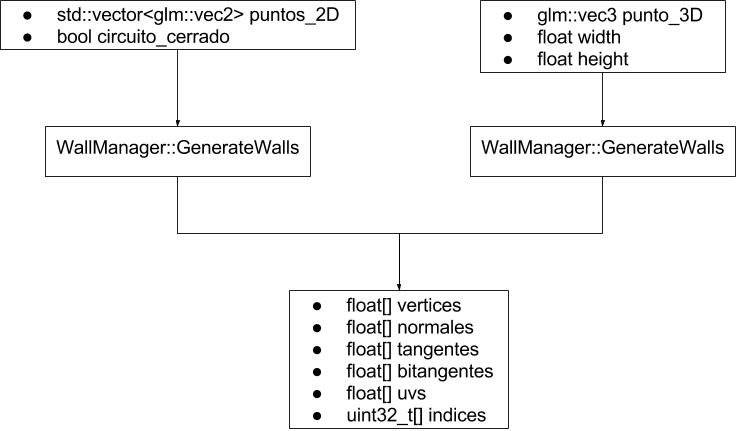
\includegraphics[width=0.75\linewidth]{I_O_ventanas}
    \caption{Nuevo input y output de GenerateWalls, incluyendo ventanas.}
    \label{fig:io_generatewindows}
\end{figure}

Para empezar se deben adaptar las paredes que ya generadas. Es conveniente que la generación de ventanas se limite a trabajar sobre un solo plano, de modo que se eliminarán los planos anterior y posterior de la pared para añadirlos después con la nueva geometría. Aunque intuitivamente pueda parecer que esto supone simplificar la geometría respecto a lo que se ha hecho hasta ahora, en realidad se complica sensiblemente. Los planos anterior y posterior de la pared van a ser siempre idénticos, pero el plano posterior es algo más alargado debido a la geometría de las esquinas que se puede apreciar en la figura \ref{fig:nomenclatura_vertices}.

\begin{figure}[H]
    \centering
    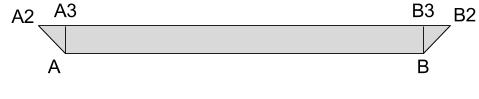
\includegraphics[width=0.75\linewidth]{Nomenclaturas_vertices_2}
    \caption{Nomenclatura final de los vértices.}
    \label{fig:nomenclatura_vertices_2}
\end{figure}

Con la nueva geometría presentada en la figura \ref{fig:nomenclatura_vertices_2} las paredes se convierten en dos prismas triangulares unidos por dos planos superior e inferior de la pared. Con esto se consigue que los planos anterior y posterior que ahora le faltan a la pared sean totalmente idénticos aunque con las normales invertidas. Esto, sin embargo, complica las conexiones entre los vértices, que se han tenido que generar manualmente. Con los nuevos vértices añadidos en total hay 35 vértices.

\begin{figure}[H]
    \centering
    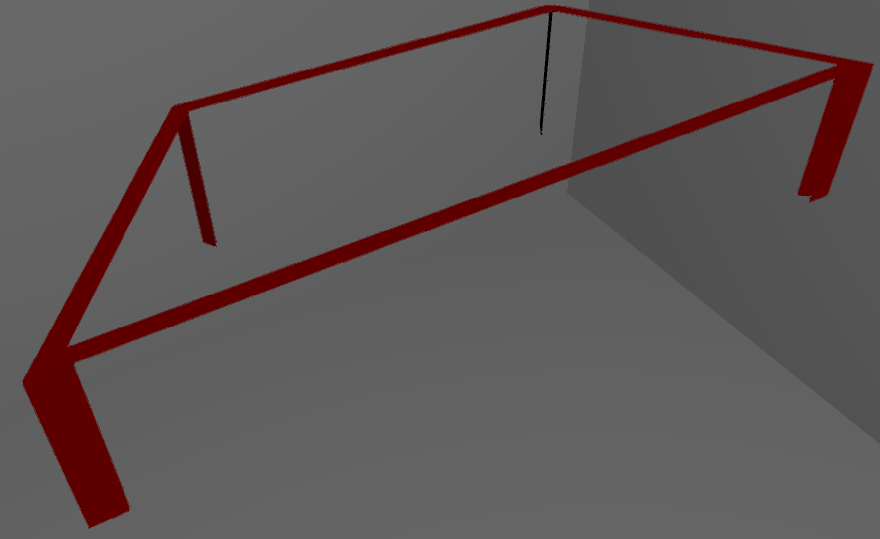
\includegraphics[width=0.75\linewidth]{paredes_frame}
    \caption{Aspecto de las paredes sin los planos anterior y posterior.}
    \label{fig:nueva_estructura}
\end{figure}

En la figura \ref{fig:nueva_estructura} puede verse el resultado. Nótese que los planos inferiores no se ven porque sus normales apuntan hacia abajo y el motor gráfico los oculta como optimización. Al crear los índices se ha tenido en cuenta el orden de estos, pues afecta al cálculo de las normales de los vértices.

%%%%%%%%%%%%%%%%%%%%%%%%%%%%%%%%%%%%%%%%%%%%%%%%%%%%%%%%%%%%%%%%%%%%%%%%%%%%%
%%%%%%%%%%%%%%%%%%%%%%%%%%%%%%%%%%%%%%%%%%%%%%%%%%%%%%%%%%%%%%%%%%%%%%%%%%%%%
%%%%%%%%%%%%%%%%%%%%%%%%%%%%%%%%%%%%%%%%%%%%%%%%%%%%%%%%%%%%%%%%%%%%%%%%%%%%%
%\clearpage
\subsection{Generación de ventanas I: proyección sobre pared}
\label{sec:wallgenwindowsi}
Como ya se ha mencionado en el apartado \ref{subsec:gen2}, las ventanas están definidas por un punto, una altura y un ancho. No se incluye ninguna información respecto a que pared es la que va a contener dicha ventana; por lo que se cogerá la pared más cercana al punto dado.

Para ello se proyecta el punto sobre la línea $AB$ de cada una de las paredes, calculando la distacia hasta cada una de las proyecciones para ver cuál es la más cercana (véase el apéndice \ref{sec:pointrayproj} sobre la proyección punto-línea):

\begin{lstlisting}
findWall(punto):
    VARIABLE pared_proxima
    VARIABLE distancia_menor
    VARIABLE distancia
    
    pared_proxima = -1
    distancia_menor = -1.0
    
    POR CADA ELEMENTO EN paredes, i:
        VARIABLE proyeccion
        proyeccion = proyeccion_punto_linea(pared[i].A1, pared[i].B1, punto)
        
        SI proyeccion encontrada ENTONCES:
            distancia = LOGITUD DE VECTOR (proyeccion - punto)
            SI distancia_menor ES MENOR QUE 0.0 O distancia < distancia_menor ENTONCES:
                distancia_menor = distancia
                pared_proxima = i
            FINSI
        FINSI
    FINPOR
    DEVOLVER pared_proxima
FIN DE FUNCION
\end{lstlisting}

Todas las ventanas o puertas han de ser necesariamente rectangulares. Esta es una precondición que se ha impuesto desde desarrollo para simplificar el cálculo de los agujeros, dado que es más sencillo incorporar geometrías más complejas incluyendo paredes falsas dentro del modelo de la ventana o puerta. Por ejemplo, si en algún momento se deseara incorporar una ventana redonda, sería más sencillo incluir 4 esquinas de pared a la ventana permitiendo que el hueco sea rectangular igualmente.

Como preparación para el próximo apartado (\ref{sec:wallgenwindowsii}) se calcula sobre la pared los 4 puntos que delimitarán la ventana. Para ello se proyecta el punto de la pared sobre el plano que forma esta, y se calcula el resto de puntos desplazándonos por dicho plano (véase el apéndice \ref{sec:pointplaneproj} sobre la proyección punto-rectángulo):

\begin{lstlisting}
projectVertices(pared, referencia a hueco):
    VARIABLE direccion_A1B1
    VARIABLE direccion_A1A1H
    VARIABLE origen
    
    direccion_A1B1 = NORMALIZAR (pared.B1 - pared.A1)
    direccion_A1A1H = NORMALIZAR (pared.A1H - pared.A1)
    
    origen = proyeccion_punto_rectangulo(pared.A1, pared.B1, pared.A1H, hueco.origen)
    
    hueco.A1 = origen
    hueco.B1 = origen + direccion_A1B1 * hueco.ancho
    hueco.A1H = origen + direccion_A1A1H * hueco.alto
    hueco.B1H = hueco.A1H + direccion_A1B1 * hueco.ancho
FIN DE FUNCION
\end{lstlisting}

%%%%%%%%%%%%%%%%%%%%%%%%%%%%%%%%%%%%%%%%%%%%%%%%%%%%%%%%%%%%%%%%%%%%%%%%%%%%%
%%%%%%%%%%%%%%%%%%%%%%%%%%%%%%%%%%%%%%%%%%%%%%%%%%%%%%%%%%%%%%%%%%%%%%%%%%%%%
%%%%%%%%%%%%%%%%%%%%%%%%%%%%%%%%%%%%%%%%%%%%%%%%%%%%%%%%%%%%%%%%%%%%%%%%%%%%%
\subsection{Generación de ventanas II: modificación de la geometría de la pared}
\label{sec:wallgenwindowsii}

Al final del apartado \ref{sec:wallgenwindowsii}, ya se conoce el punto en que están los extremos de la ventana sobre la pared. En este apartado se explica cómo dividir la pared en diferentes planos y descartar aquellos que correspondan a un agujero.

Una vez más las proyecciones cobran mucho protagonismo (véase el apéndice \ref{sec:pointrayproj} sobre la proyección punto-línea). Lo primero que se busca es dividir el plano de la pared por los vértices del hueco, obteniendo una colección de planos como se puede ver en la figura \ref{fig:wall_separacion}.

\begin{figure}[H]
    \centering
    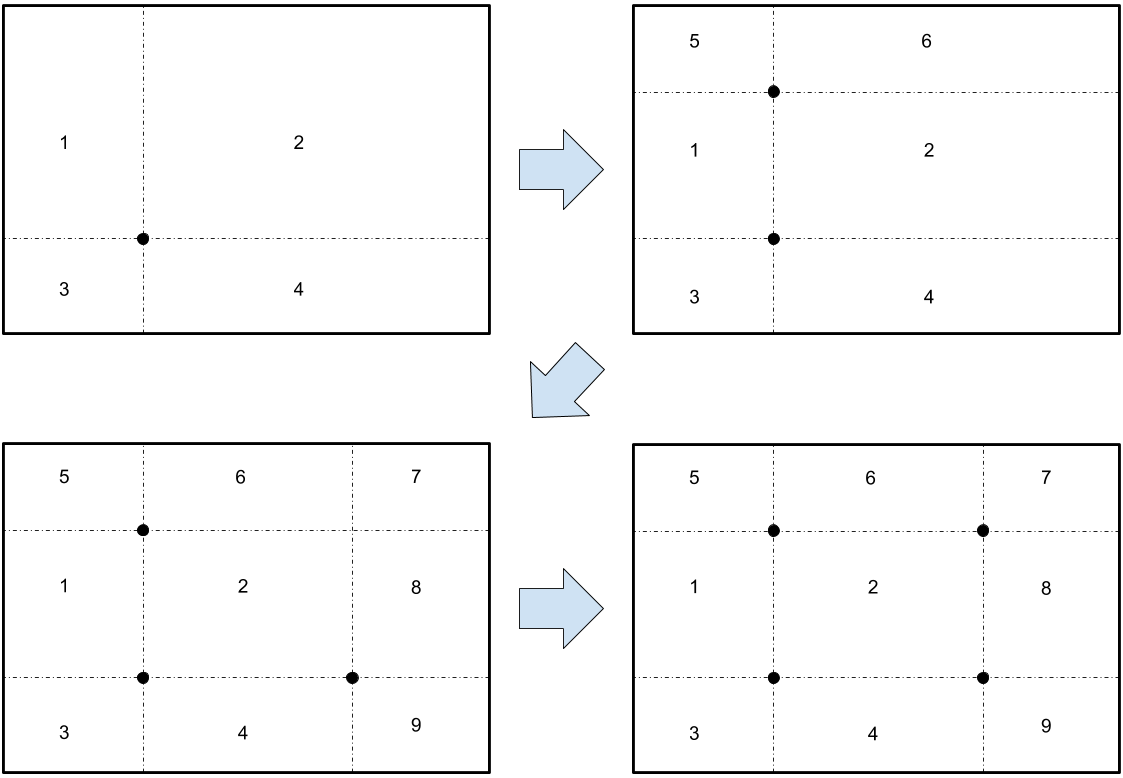
\includegraphics[width=0.85\linewidth]{Separaciones_paredes}
    \caption{Separación de la pared en planos}
    \label{fig:wall_separacion}
\end{figure}

El algoritmo para conseguir esto tiene como entrada y salida una lista de planos, que empieza siendo uno solo que cubre toda la pared. Mientras iteramos los puntos, proyectamos estos sobre cada lado para obtener los puntos por los que hay que cortar los planos, y posteriormente se añaden a la lista de planos desechando el original. En caso de que una de las proyecciones no contribuya a crear un nuevo plano (como por ejemplo, los puntos inferiores de la puerta en la figura \ref{fig:mult_and_red_windows}) la ignoramos.

Posteriormente se comprueba cuales de estos planos forman parte de una ventana y se eliminan de la lista, dejando un hueco en dicha posición. Este algoritmo permite además añadir múltiples ventanas, aumentando la posible complejidad de la pared.

Por último se reprocesan los planos generados comprobando si sus lados coinciden en alguna dirección, en cuyo caso se reúnen para reducir la complejidad. En la figura \ref{fig:mult_and_red_windows}, se puede ver un ejemplo de como se separan los planos con múltiples ventanas, y cómo se reúnen los planos adyacentes.

\begin{figure}[H]
    \centering
    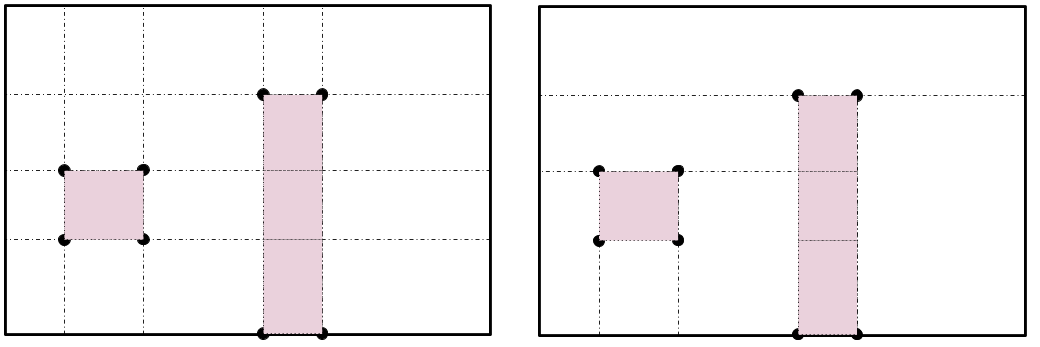
\includegraphics[width=0.85\linewidth]{mult_window_and_reduction}
    \caption{Ejemplo de pared con una ventana y una puerta, y muestra de una posible reducción de los planos.}
    \label{fig:mult_and_red_windows}
\end{figure}

\begin{figure}[H]
    \centering
    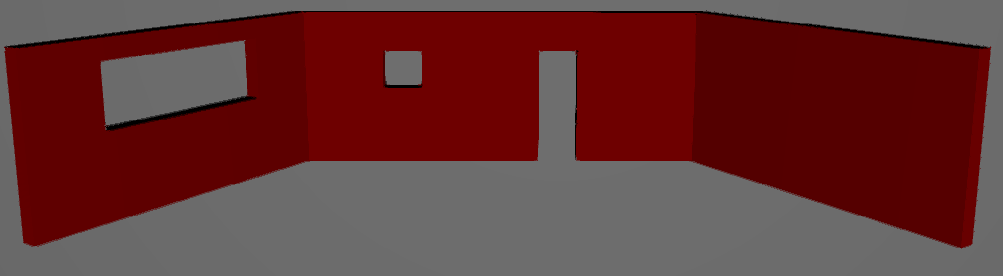
\includegraphics[width=0.85\linewidth]{Agujeros}
    \caption{Ejemplo de generación de paredes con huecos y estancia sin cerrar.}
    \label{fig:wall_with_window_example}
\end{figure}

%%%%%%%%%%%%%%%%%%%%%%%%%%%%%%%%%%%%%%%%%%%%%%%%%%%%%%%%%%%%%%%%%%%%%%%%%%%%%
%%%%%%%%%%%%%%%%%%%%%%%%%%%%%%%%%%%%%%%%%%%%%%%%%%%%%%%%%%%%%%%%%%%%%%%%%%%%%
%%%%%%%%%%%%%%%%%%%%%%%%%%%%%%%%%%%%%%%%%%%%%%%%%%%%%%%%%%%%%%%%%%%%%%%%%%%%%
\subsection{Generación de uvs}
Para que el motor aplique correctamente las texturas sobre las paredes, se requiere que las uvs estén a escala de mundo; es decir, se espera que dada una distancia entre dos vértices de la mima malla, sus uvs tengan la misma distancia. La mayor dificultad en este caso está en que los vértices se encuentran en espacio tridimensional, mientras que las uv son coordenadas bidimensionales de la textura que estamos mapeando. Por lo tanto, de algún modo hay que desconsiderar la orientación de la pared y centrarnos en sus superficies.

Como la geometría está formada por planos perfectos, la solución encontrada ha consistido en partir siempre de la esquina inferior izquierda de cada uno de ellos. Como precondición, la esquina ``A" tiene la uv (0,0).

Por lo tanto por cada plano, se ha definido la uv de la esquina inferior izquierda, y los vectores hacia los cuales ``avanzan" las componentes \texttt{x} e \texttt{y} de las uv (Fig. \ref{fig:datos_uvs}).

\begin{figure}[H]
    \centering
    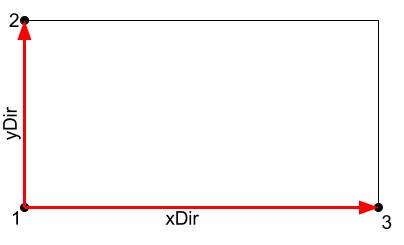
\includegraphics[scale=0.75]{Datos_uvs}
    \caption{Datos necesarios para la generación de las uv ``2" y ``3".}
    \label{fig:datos_uvs}
\end{figure}

La razón de usar proyecciones y no la magnitud de los vectores directamente, es que se desconoce en cual de las dos direcciones se encuentra el vértice que observamos al iterar. Proyectando cada punto tenemos la distancia en cada una de las dos direcciones y se la sumamos a la uv del vértice ``1":

\begin{lstlisting}
genUV(origen, xDir, yDir, punto, uv_origen, longitud_x, longitud_y):
    VARIABLE uv COMO VECTOR 2D
    uv.x = proyeccion_punto_rayo(origen, xDir, punto)
    uv.y = proyeccion_punto_rayo(origen, yDir, punto)
    
    SI longitud_x > 0.0 Y uv.x < 0.0 ENTONCES:
        uv.x = longitud_x - uv.x
    FINSI
    SI longitud_y > 0.0 Y uv.y < 0.0 ENTONCES
        uv.y = longitud_y - uv.y
    FINSI
    
    uv = uv + uv_origen
    DEVOLVER uv
FIN DE FUNCION
\end{lstlisting}

Dado que las uv no pueden ser negativas, se hace un paso en las líneas 6-11 para que, en caso de serlo, se les sume la longitud total del lado en el que se encuentran.

%%%%%%%%%%%%%%%%%%%%%%%%%%%%%%%%%%%%%%%%%%%%%%%%%%%%%%%%%%%%%%%%%%%%%%%%%%%%%
%%%%%%%%%%%%%%%%%%%%%%%%%%%%%%%%%%%%%%%%%%%%%%%%%%%%%%%%%%%%%%%%%%%%%%%%%%%%%
%%%%%%%%%%%%%%%%%%%%%%%%%%%%%%%%%%%%%%%%%%%%%%%%%%%%%%%%%%%%%%%%%%%%%%%%%%%%%
\subsection{Generación de normales, tangentes y bitangentes}
El cálculo de cada normal es el resultado de la suma de la normal de cada polígono en el que se encuentra dicho vértice, y para calcular esta se hace el producto vectorial (normalizado) de los vectores que van del primer vértice hacia el segundo y el tercero:

\begin{lstlisting}
VARIABLES EXTERNAS v1, v2, v3

normal = NORMALIZAR ( PRODUCTO CRUZADO DE (v2 - v1) Y (v3 - v1))
\end{lstlisting}

Las tangentes y bitangentes son un poco más complicadas: todo vector tiene infinitos vectores tangentes, pero en este caso no sirve cualquiera. El vector tangente a la normal tiene que estar siempre alineado con las uv.

Como se explica en el tutorial 13 de opengl-tutorial.org \footfullcite{opengltutorials}, para ello debemos resolver el siguiente sistema de ecuaciones:


\[ deltaPos1 = deltaUV1.x * T + deltaUV1.y * B \]
\[ deltaPos2 = deltaUV2.x * T + deltaUV2.y * B \]

Esto se computar como

\begin{lstlisting}
VARIABLES EXTERNAS uv1, uv2, uv3, v1, v2, v3

VARIABLES vec1, vec2
vec1 = v2 - v1
vec2 = v3 - v1

VARIABLES deltaUV1, deltaUV2 COMO VECTORES 2D
deltaUV1 = uv2 - uv1
deltaUV2 = uv3 - uv1

VARIABLE r
r = 1.0 / (deltaUV1.x * deltaUV2.y - deltaUV1.y * deltaUV2.x)

VARIABLES tangente, bitangente
tangente = (vec1 * deltaUV2 - vec2 * deltaUV1.y) * r
bitangente = (vec2 * deltaUV1.x - vec1 * deltaUV2.x) * r
\end{lstlisting}
